\chapter{Gesichtserkennung}
\textit{Erarbeitet von Marco Kuner.} \\

\noindent
Diese Dokumentation beschreibt die Entwicklung einer Gesichtserkennungslösung für einen Smart Mirror. Das Projekt wurde im Rahmen eines Vier-Personen-Teams durchgeführt und beinhaltet die Recherche, Implementierung und Optimierung verschiedener Gesichtserkennungstechnologien. Besonderes Augenmerk liegt auf der genauen Protokollierung der Entscheidungsprozesse und der technischen Herausforderungen.

\section{Einleitung}

\subsection{Projektziel}
Das Hauptziel dieses Projekts war die Entwicklung einer fortschrittlichen Gesichtserkennungslösung für einen Smart Mirror. Dieser Smart Mirror sollte in der Lage sein, Benutzer anhand ihrer Gesichter zu erkennen und personalisierte Informationen anzuzeigen. Die Gesichtserkennung sollte zuverlässig unter verschiedenen Bedingungen wie wechselnden Lichtverhältnissen und unterschiedlichen Gesichtswinkeln funktionieren.

\subsection{Bedeutung der Gesichtserkennung}
Gesichtserkennungstechnologien haben in den letzten Jahren erheblich an Bedeutung gewonnen. Sie finden Anwendungen in zahlreichen Bereichen wie Sicherheit, wo sie zur Zugangskontrolle und Überwachung eingesetzt werden, in der Personalisierung, wo sie individuelle Benutzererlebnisse ermöglichen, und in der Benutzerfreundlichkeit, da sie eine nahtlose Interaktion mit technischen Geräten bieten. Die Entwicklung einer zuverlässigen Gesichtserkennung für den Smart Mirror ist also zwingend erforderlich für eine reibungslose Kundenerfahrung.



\section{Recherche und Anfangsphase}

\subsection{Grundlagen der Gesichtserkennung}
Gesichtserkennung ist ein Bereich der Computer Vision, der sich mit der Identifikation von Individuen anhand ihrer Gesichtszüge beschäftigt. Dies geschieht durch den Einsatz von Algorithmen, die charakteristische Merkmale eines Gesichts extrahieren und analysieren. Traditionelle Methoden der Gesichtserkennung umfassen Ansätze wie die Verwendung von Haar-Cascades, während moderne Methoden oft auf tiefen neuronalen Netzwerken basieren.

\subsection{Vergleich von Methoden}
In der Anfangsphase des Projekts wurde zunächst die Möglichkeit in Betracht gezogen, ein eigenes Deep-Learning-Modell für die Gesichtserkennung zu trainieren. Nach weiterer Recherche und intensiver Absprache mit Kommilitonen aus dem KI-Studiengang wurde jedoch festgestellt, dass das Training eines eigenen Modells aufgrund des hohen Zeitaufwands und der benötigten Rechenressourcen nicht praktikabel wäre.

\noindent Daraufhin wurde eine umfassende Recherche zu verschiedenen existierenden Methoden der Gesichtserkennung durchgeführt. Dabei wurden herkömmliche Ansätze wie Haar-Cascades und moderne Ansätze wie Deep Learning verglichen. Haar-Cascades, die auf der Viola-Jones-Methode basieren, bieten den Vorteil einer schnellen Berechnung und einfachen Implementierung, sind jedoch in ihrer Genauigkeit und Robustheit begrenzt. Im Gegensatz dazu bieten moderne Deep-Learning-Ansätze, wie sie in der Dlib-Bibliothek verwendet werden, eine höhere Genauigkeit und Robustheit, erfordern jedoch mehr Rechenleistung und sind komplexer in der Implementierung.



\section{Erste Implementierung mit Haar-Cascades}

\subsection{Haar-Cascade-Ansatz}
Aufgrund des begrenzten Speichers unseres Raspberry Pi wurde zunächst der Haar-Cascade-Ansatz gewählt, da dieser deutlich weniger komplex aufgebaut ist und weniger Rechenleistung erfordert. Haar-Cascades basieren auf der Viola-Jones-Methode, die einen robusten Algorithmus zur Gesichtserkennung darstellt. 

\noindent Die Haar-Cascade-Methode verwendet eine Kaskade von sogenannten Haar-ähnlichen Merkmalen\cite{haar_quelle}. Eine Kaskade in diesem Kontext bedeutet eine Abfolge von Klassifikatoren, die nacheinander angewendet werden, um die Erkennungsgenauigkeit zu erhöhen und gleichzeitig die Rechenleistung zu optimieren. Diese Merkmale sind einfache Muster, die in unterschiedlichen Größen und Positionen auf das Bild angewendet werden, um Kontraste zu erkennen, die typisch für Gesichtszüge sind. \\ \\

\begin{figure}[h!]
    \centering
    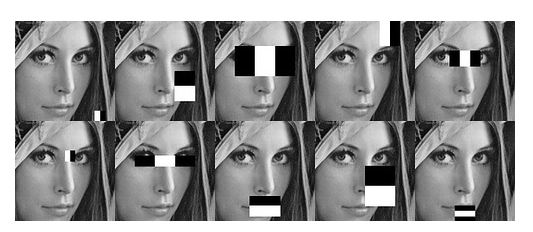
\includegraphics[width=0.5\textwidth]{pictures/haarcascades.jpg}
    \caption{Beispiel verschiedener Haar-ähnlicher Merkmale}
    \label{fig:haar_cascade_example}
    \cite{haar_cascade_example}
\end{figure} 

\noindent Ein integrales Bild wird verwendet, um diese Merkmale effizient zu berechnen. Die Viola-Jones-Methode besteht aus mehreren Hauptkomponenten:\\

\noindent \textbf{Merkmalserkennung}: Haar-ähnliche Merkmale bestehen aus einfachen rechteckigen Bereichen, die Intensitätsunterschiede innerhalb des Bildes messen. Es gibt drei Arten von Haar-ähnlichen Merkmalen: Kantenmerkmale, Linienmerkmale und vierrechteckige Merkmale. Diese Merkmale helfen dabei, grundlegende Strukturen wie Kanten, Linien und Ecken zu erfassen, die in Gesichtern häufig vorkommen. \\

\noindent \textbf{Integralbild}: Das Integralbild ist eine Datenstruktur, die verwendet wird, um die Berechnung von Rechteckmerkmalen in konstanter Zeit zu ermöglichen. Dies wird erreicht, indem für jedes Pixel die Summe aller Pixelwerte oben und links davon berechnet wird. Dadurch kann jedes Rechteckmerkmal durch wenige Zugriffe auf das Integralbild effizient berechnet werden. \\

\noindent \textbf{Adaboost-Training}: Um die Merkmale zu einem starken Klassifikator zu kombinieren, wird der Adaboost-Algorithmus verwendet. Adaboost ist eine Methode des maschinellen Lernens, die eine große Anzahl schwacher Klassifikatoren zu einem starken Klassifikator kombiniert. Während des Trainingsprozesses werden die wichtigsten Merkmale ausgewählt und gewichtet, um die Erkennungsrate zu maximieren und gleichzeitig die Fehlerrate zu minimieren.\\

\noindent \textbf{Kaskadenklassifikation}: Die Klassifikatoren werden in einer Kaskade organisiert, wobei jeder Klassifikator die Aufgabe hat, ein Fenster entweder als Gesicht oder Nicht-Gesicht zu klassifizieren. Ein Fenster, das von einem Klassifikator als Nicht-Gesicht klassifiziert wird, wird sofort verworfen, was die Berechnungen erheblich beschleunigt. Nur Fenster, die von allen Klassifikatoren in der Kaskade als Gesicht erkannt werden, werden letztendlich als Gesicht klassifiziert.\\

\noindent Die ersten Versuche konzentrierten sich darauf, Gesichter in verschiedenen Beleuchtungssituationen und Winkeln zu erkennen, um die Robustheit des Ansatzes zu testen.


\subsection{Vorteile und Nachteile}
Nach der Implementierung des Haar-Cascade-Ansatzes in OpenCV wurde die Methode intensiv getestet, um ihre Vor- und Nachteile zu ermitteln: \\

\noindent \textbf{Vorteile}:
\begin{itemize}
    \item \textbf{Schnelle Berechnung}: Die Methode ist sehr effizient in der Berechnung und kann in Echtzeit auf Geräten mit begrenzten Ressourcen wie dem Raspberry Pi ausgeführt werden.
    \item \textbf{Einfache Implementierung}: OpenCV bietet vorgefertigte Haar-Cascade-Modelle, die leicht zu integrieren sind.
\end{itemize}

\noindent \textbf{Nachteile}:
\begin{itemize}
    \item \textbf{Begrenzte Genauigkeit}: Die Genauigkeit der Erkennung ist begrenzt, insbesondere bei schwierigen Lichtverhältnissen oder seitlich aufgenommenen Gesichtern.
\end{itemize}

\subsection{Ergebnisse der Tests}

 Der Problem lag in der mangelhaften Genauigkeit, insbesondere bei schwierigen Lichtverhältnissen oder seitlich aufgenommenen Gesichtern. Diese Einschränkung lässt sich dadurch erklären, dass Haar-Cascades stark auf Kontraste und einfache geometrische Merkmale angewiesen sind. Bei wechselnden Lichtverhältnissen ändern sich die Intensitätsunterschiede im Bild, was dazu führt, dass die Merkmale, die für die Erkennung verwendet werden, weniger zuverlässig sind. Dies beeinträchtigt die Genauigkeit der Erkennung erheblich, da die Algorithmen Schwierigkeiten haben, die relevanten Merkmale konsistent zu identifizieren.

\noindent Zusammenfassend zeigte sich, dass die Haar-Cascade-Methode zwar effizient in der Berechnung ist und schnell auf Geräten mit begrenzten Ressourcen wie dem Raspberry Pi ausgeführt werden kann, jedoch nicht die erforderliche Präzision und Robustheit für die Gesichtserkennung in einem Smart Mirror bietet. Diese Erkenntnisse führten zur Entscheidung, nach präziseren Methoden für die Gesichtserkennung zu suchen.




\section{Umstieg auf Dlib für höhere Präzision}

\subsection{Wechsel zu Dlib}
Nach dem begrenzten Erfolg mit Haar-Cascades wurde entschieden, auf die Dlib-Bibliothek umzusteigen, um eine robustere Gesichtserkennung zu erreichen. Dlib ist eine freie Software-Bibliothek, die Algorithmen für maschinelles Lernen, Bildverarbeitung und maschinelles Sehen bereitstellt. Für die Gesichtserkennung in diesem Projekt wurde insbesondere der Histogram of Oriented Gradients (HOG)-Algorithmus und das 68-Facial-Landmarks-Modell zur präzisen Merkmalsextraktion verwendet.

\subsection{Technologien: HOG und 68-Facial-Landmarks}
\textbf{Histogram of Oriented Gradients (HOG)}: Der HOG-Algorithmus ist eine Methode zur Merkmalserkennung in Bildern, die darauf basiert, das lokale Auftreten von Gradientenorientierungen zu zählen. Der HOG-Algorithmus bildet die Basis des vortrainierten 68-facial-landsmarks-Modells. Diese Methode funktioniert folgendermaßen:

\begin{itemize}
    \item \textbf{Gradientenberechnung}: Für jedes Pixel im Bild wird der Gradient berechnet. Der Gradient eines Pixels gibt die Richtung und die Stärke der größten Helligkeitsänderung an\cite{hog_quelle}. Dies geschieht durch die Anwendung von Sobel-Filtern in horizontaler und vertikaler Richtung, wodurch zwei Bilder entstehen, die die Helligkeitsänderungen in x- und y-Richtung darstellen. Der Gradient kann dann durch die Kombination dieser beiden Bilder berechnet werden.
    
    \item \textbf{Zellaufteilung}: Das Bild wird in kleine Zellen unterteilt, typischerweise von 8x8 Pixeln. Diese Zellen sind klein genug, um lokale Details zu erfassen, aber groß genug, um signifikante Informationen zu enthalten. Innerhalb jeder Zelle werden die Gradientenorientierungen der Pixel gesammelt und analysiert.
    
    \item \textbf{Orientierungshistogramme}: Für jede Zelle wird ein Histogramm der Gradientenorientierungen erstellt. Die Gradienten innerhalb jeder Zelle werden in Bins sortiert, die verschiedene Richtungen repräsentieren, üblicherweise in 9 Bins, die Winkelbereiche von 0 bis 180 Grad abdecken. Jeder Bin enthält die Summe der Gradientenstärken, die in seine Richtung fallen, was eine robuste Darstellung der Orientierungsmuster innerhalb der Zelle ermöglicht.
    
    \item \textbf{Normierung}: Um die Beleuchtungsunterschiede zu kompensieren, werden die Histogramme in Blöcken normalisiert. Ein Block besteht aus mehreren benachbarten Zellen, typischerweise 2x2. Die Normierung erfolgt durch Berechnung der Quadratwurzel der Summe der quadrierten Bin-Werte, was eine gleichmäßige Darstellung der Merkmale ermöglicht, unabhängig von lokalen Beleuchtungsunterschieden.
    
    \item \textbf{Merkmalsvektor}: Die normalisierten Histogramme aller Blöcke werden zu einem einzigen Merkmalsvektor zusammengefügt, der das Bild repräsentiert. Dieser Merkmalsvektor ist hochdimensional und enthält eine detaillierte Beschreibung der Gradientenorientierungen im gesamten Bild. Er dient als Eingabe für maschinelle Lernalgorithmen, die darauf trainiert sind, Gesichter von Nicht-Gesichtern zu unterscheiden.
\end{itemize}

\begin{figure}[h!]
    \centering
    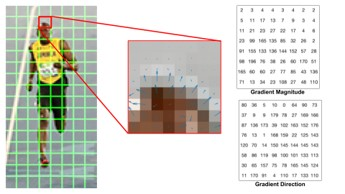
\includegraphics[width=0.5\textwidth]{pictures/hog.jpg}
    \caption{Beispiel einer HOG-Analyse}
    \label{fig:hoganalysis}
    \cite{hoganalysis}
\end{figure}


\subsection{Implementierung und Herausforderungen}
Die Implementierung von Dlib für die Gesichtserkennung begann mit der Integration der Bibliothek und dem Einbinden der vortrainierten Modelle für HOG und Facial Landmarks. Dies stellte sich jedoch als Herausforderung heraus, da Dlib zwei große Dateien (68-Landmarks-Modell: ca. 100MB; ResNet-Modell: ca. 21MB) benötigt, die die Modelle zur Gesichtserkennung und Merkmalsextraktion enthalten. Auf dem Raspberry Pi führte dies aufgrund des begrenzten RAMs von einem GB zu erheblichen Leistungsproblemen. \\ 

\noindent Die Implementierung der Gesichtserkennung erfolgte durch die `main.py`, welche die folgenden Hauptschritte umfasst:

\begin{itemize}
    \item \textbf{Initialisierung und Laden der Modelle}: Zunächst wurden die notwendigen Modelle geladen, darunter der Frontalgesicht-Detektor, das 68-Landmarks-Modell und das ResNet-Modell zur Gesichtserkennung und -extraktion. Diese Modelle wurden verwendet, um Gesichter im Videostream zu erkennen und deren Merkmale zu extrahieren.
    \item \textbf{Starten der WebSocket-Verbindung}: Eine WebSocket-Verbindung wurde initialisiert, um die Profile zwischen dem Smart Mirror und der mobilen Kontroll-App zu synchronisieren.
    \item \textbf{Erfassung und Verarbeitung des Videostreams}: Der Videostream wurde von der Kamera erfasst und in Graustufen umgewandelt, um die Gesichtserkennung zu erleichtern. Die Erkennung der Gesichter erfolgte durch den Frontalgesicht-Detektor.
    \item \textbf{Erkennung und Markierung der Gesichtspunkte}: Sobald ein Gesicht erkannt wurde, wurden die 68 Gesichtspunkte (Landmarks) ermittelt. Diese Landmarks dienten als Grundlage für die weitere Merkmalsextraktion.
    \item \textbf{Merkmalsextraktion mit dem ResNet-Modell}: Basierend auf den ermittelten Landmarks wurde das Face Embedding mit dem ResNet-Modell berechnet. Dieses Modell erzeugte einen 128-dimensionalen Vektor, der die einzigartigen Merkmale des Gesichts repräsentiert.
    \item \textbf{Gesichtserkennung und Profilsynchronisation}: Das erzeugte Face Embedding wurde verwendet, um das Gesicht zu erkennen oder ein neues Profil zu erstellen. Diese Informationen wurden anschließend gespeichert und über die WebSocket-Verbindung synchronisiert (die Logik für die Feature Extraction, das Abgleichen der Face Embeddings und die Profil- und Synchronisationslogik wird in späteren Kapiteln ausführlicher erklärt).
    \item \textbf{Anzeige der Ergebnisse}: Das erkannte Gesicht und die entsprechenden Landmarks wurden im Videostream hervorgehoben und mit dem erkannten Profilnamen versehen.
\end{itemize}

\noindent In seltenen Fällen trat ein Segmentation Fault auf, vermutlich weil der Stack im RAM aufgrund der umfassenden Modelle zu groß wurde. Es trat nur sporadisch auf, sodass es in der weiteren Entwicklung hintenangestellt wurde.


\subsection{Verbesserung der Performance}
Die initiale Implementierung mit Dlib ergab in qualifizierten Tests eine Performance von maximal einer Ausführung pro Sekunde. Um die Performance zu verbessern, wurden verschiedene Techniken implementiert:

\begin{itemize}
    \item \textbf{Reduzierung der Bildgröße}: Durch die Reduzierung der Bildgröße vor der Verarbeitung soll die Berechnungszeit verringert werden.
    \item \textbf{Frame Skipping}: Nicht jeder Frame wurde überprüft, um die Verarbeitungslast zu reduzieren.
    \item \textbf{Multithreading}: Implementierung von Multithreading zur gleichzeitigen Verarbeitung mehrerer Aufgaben.
\end{itemize}

\noindent Trotz Implementierung all dieser Techniken konnte die Performance auf nur maximal zwei Ausführungen pro Sekunde angehoben werden. Die Lösung kam letztendlich durch einen Rat von Professor Metzner: "[...]Es ist egal, dass es so langsam läuft, eine Gesichtsabfrage 1 mal pro Sekunde ist völlig ausreichend.[...]" Diese pragmatische Einstellung ermöglichte es mir, mich auf die Feature Extraction zu konzentrieren, anstatt auf die Geschwindigkeit der Gesichtserkennung. 


\section{Feature Extraction und Matching}

\subsection{Feature Extraction}
Um zu überprüfen, ob ein Gesicht neu oder bereits im System bekannt ist, wurde Dlib's Deep Metric Learning Ansatz verwendet. Dieser Ansatz dient der Feature Extraction und nutzt das ResNet-Modell, das speziell für die Gesichtserkennung trainiert wurde.

\noindent \textbf{Vorgehensweise}:
\begin{itemize}
    \item \textbf{Landmark-Detektion}: Nach der Gesichtserkennung werden relevante Gesichtspunkte mittels des vorher bereits erwähnten Modells bestimmt. Dieses vortrainierte ML-Modell erkennt 68 charakteristische Punkte im Gesicht, wie Augen, Nase, Mund und Kieferlinie. Diese Punkte werden als Landmarks bezeichnet und helfen dabei, die Position und Ausrichtung des Gesichts zu bestimmen und dienen als Eingabe in das ResNet-Modells.
    
    \item \textbf{Berechnung des Gesichtsembeddings}: Mit Hilfe des Dlib-ResNet-Modells wird aus den extrahierten Landmarken ein Gesichtsembedding berechnet. Das ResNet-Modell verwendet die Informationen der 68 Landmarks, um einen 128-dimensionalen Vektor zu erzeugen. Dieser Vektor, das sogenannte Gesichtsembedding, repräsentiert die einzigartigen Merkmale eines Gesichts in einem hochdimensionalen Raum. Die Werte des Vektors sind als Floating Points zwischen 0 und 1 skaliert.
\end{itemize}

\begin{figure}[h!]
    \centering
    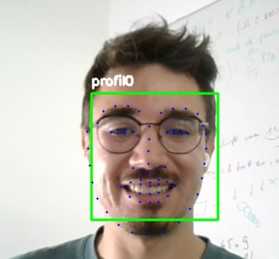
\includegraphics[width=0.5\textwidth]{pictures/68landmarks.jpg}
    \caption{Praxisbeispiel der 68-landmarks}
    \label{fig:68landmarks}
    \cite{68landmarks}
\end{figure}

\subsection{Vergleich der Gesichtsembeddings}
Die erstellten Embeddings werden zur Identifikation von Personen genutzt, indem sie mit bereits gespeicherten Embeddings verglichen werden. \\

\noindent \textbf{Vergleichsmethode}:
Zur Identifikation wird der euklidische Abstand zwischen den Embeddings berechnet. Der euklidische Abstand ist eine Maßzahl für die Distanz zwischen zwei Punkten in einem n-dimensionalen Raum, die durch die Wurzel der Summe der quadrierten Differenzen ihrer Koordinaten berechnet wird. Wenn der Abstand gering ist (unter einem bestimmten Schwellenwert, z.B. 0.6), wird angenommen, dass es sich um dieselbe Person handelt. Der Schwellenwert von 0,6 wurde durch eine Reihe von Tests empirisch bestimmt, um eine Balance zwischen False Positives und False Negatives zu erreichen, was eine zuverlässige Unterscheidung zwischen verschiedenen Personen ermöglichen soll.

\section{Speichern und Verwalten der Profile}

An diesem Zeitpunkt im Projekt war der Kern der Gesichtserkennung, also das Erkennen eines Gesichts, das Erstellen eines Face Embeddings und die Logik für den Vergleich mit bereits erkannten Gesichtern, fertiggestellt. Es folgte also nun die Integration in unser bestehendes System. Die Kommunikation mit dem Display-Webserver lief reibungslos, da dieser auf dem gleichen Gerät gehostet wird und somit nur der Ablagepfad der Profildaten geändert werden musste. Ein größeres Problem war jedoch die Kommunikation mit der Remote-App. Da diese ebenfalls Änderungen an den Profilen vornehmen kann, mussten wir sicherstellen, dass die Profile samt Einstellungen auf beiden Seiten synchron sind, um Informationsverlust oder Schlimmeres zu verhindern. Dafür gab es einige Besprechungen mit dem Entwickler der App, David Vollmer. Wir einigten uns auf ein genormtes Format der Profildatenspeicherung (profiles.json), welches dann über einen Websocket vom Spiegel an die Remote und vice versa gesendet werden kann.
\subsection{Speichern der Profile}
 Wenn ein unbekanntes Gesichtsembedding identifiziert wird, wird ein neues Profil mit Standardwerten in der JSON-Datei erstellt. Diese Datei enthält die Informationen darüber, welche Profile existieren, welches Profil gerade aktiv ist und für jedes Profil, welche Widgets (IDs) an welcher Stelle (index) angezeigt werden sollen. Wird ein Gesichtsembedding wiedererkannt, wird jediglich das dazugehörige 'isSelected' Flag gesetzt und das vorherige gecleared.


\subsection{Verbindung zum Websocket}
Um die Profile mit der Android-Remote zu synchronisieren wurde eine Websocket-Verbindung implementiert. Diese Verbindung ermöglicht die Echtzeitsynchronisation von Profiländerungen zwischen dem Smart Mirror und der Android-App.

\noindent \textbf{Vorgehensweise}:
\begin{itemize}
    \item \textbf{Websocket-Listener}: Sowohl die Remote-App als auch der Smart Mirror haben jeweils einen Listener am Websocket, um Nachrichten zu empfangen.
    
    \item \textbf{Synchronisation beim App-Start}: Beim Starten der Android-App sendet sie einen 'fetch'-Befehl über den Websocket, um sicherzustellen, dass sie sofort mit den aktuellen Profildaten synchronisiert wird. Der Smart Mirror antwortet daraufhin mit der aktuellen profiles.json-Datei.

    \item \textbf{Automatische Updates bei Profiländerungen}: Die profiles.json wird jedes Mal von dem Spiegel an den Websocket gesendet, wenn:
    \begin{itemize}
        \item Ein neues Profil angelegt wurde (das neue Profil erhält automatisch das 'isSelected'-Flag).
        \item Ein neues, aber bereits bekanntes Gesicht erkannt wird und das 'isSelected'-Flag entsprechend gesetzt wurde.
    \end{itemize}

    \item \textbf{Updates von der Remote-App}: Wenn die Remote-App eine Änderung an einem Profil vornimmt, sendet sie die profiles.json an den Websocket. Der Smart Mirror empfängt diese Nachricht und ersetzt die bestehende profiles.json mit den neuen Daten.
\end{itemize}

\section{Schlussfolgerung}



\subsection{Ausblick}
Die Entwicklung der Gesichtserkennungslösung hat eine solide Grundlage geschaffen, auf der zukünftige Erweiterungen und Verbesserungen aufbauen können. Obwohl einige vielversprechende Ideen aufgrund der Stabilität des Systems nicht umgesetzt wurden, bieten sie spannende Möglichkeiten für zukünftige Arbeiten.

\begin{itemize}
    \item \textbf{Age- und Gender-Classifier}: Die Dlib-Bibliothek bietet auch Age- und Gender-Classifier, die in Zusammenarbeit mit dem Widget-Team als eigenständiges Widget hätten angeboten werden können. Lokale Tests hatten dazu bereits funktioniert, und eine vollständige Implementierung könnte die Personalisierung des Smart Mirrors weiter verbessern.
    
    \item \textbf{Änderung des Profilnamens}: Mit mehr Zeit wäre eine Möglichkeit implementiert worden, den Profilnamen zu ändern. Derzeit ist der Profilname der einzigartige Bezeichner für die Face Embeddings. Um dies zu ermöglichen, müsste ein zusätzlicher eindeutiger Bezeichner eingeführt und die Profil-Logik sowohl auf dem Spiegel als auch in der App angepasst werden.
    
    \item \textbf{Flusskontrolle}: Eine weitere wichtige Verbesserung wäre die Einführung einer Flusskontrolle. Derzeit senden Spiegel und App Änderungen sofort, wenn bestimmte Ereignisse auftreten. Dies kann zu Konflikten und inkonsistenten Daten führen, wenn beide Seiten gleichzeitig senden. Eine Flusskontrolle könnte sicherstellen, dass nur eine Seite senden kann, während die andere Seite blockiert ist. Gesendete Änderungen während der Blockierphase würden in einem Puffer gespeichert und nach der Blockierung sofort gesendet.
    
    \item \textbf{Optimierung des Schwellenwerts}: Mit mehr Zeit hätten intensivere Tests zur Einstellung des euklidischen Abstands durchgeführt werden können, um Fehler wie bei der Produktpräsentation zu vermeiden. Ein genauer kalibrierter Schwellenwert könnte die Erkennungsgenauigkeit weiter verbessern und sicherstellen, dass neue Gesichter nicht fälschlicherweise als bekannte Profile erkannt werden.
    
    \item \textbf{Datenbanksynchronisation}: Wenn wir vorher gewusst hätten, wie aufwändig die Synchronisation der Profile sein würde, hätten wir definitiv eine Datenbank verwendet , die die Synchronisation eigenständig durchführt. Eine Datenbank könnte viele der aktuellen Herausforderungen bei der Datenkonsistenz und -synchronisation lösen.
\end{itemize}

\subsection{Zusammenfassung}
Im Verlauf dieses Projekts wurde eine fortschrittliche Gesichtserkennungslösung für einen Smart Mirror entwickelt. Der Übergang von herkömmlichen Haar-Cascades zu modernen Methoden wie Dlib und HOG führte zu einer signifikanten Verbesserung der Erkennungsgenauigkeit. Trotz der Performance-Probleme konnte eine zufriedenstellende Verarbeitungsgeschwindigkeit erreicht werden.

\noindent Ein wichtiger Teil des Projekts war die Speicherung und Verwaltung der Profildaten sowie die Synchronisation mit einer Android-Remote-App über eine Websocket-Verbindung. Die Trennung der Face Embeddings von der profiles.json-Datei und die Implementierung eines robusten Synchronisationsmechanismus stellten sicher, dass die Daten auf beiden Seiten konsistent und aktuell blieben.

\noindent Insgesamt konnte eine zuverlässige Gesichtserkennung und Profilverwaltung implementiert werden.
